\documentclass[12pt]{article}
\usepackage[spanish]{babel}
\usepackage{geometry}
\geometry{a4paper, margin=1in}
\usepackage{graphicx}
\usepackage{xcolor}
\usepackage{titlesec}
\usepackage{parskip}
\usepackage{multicol}
\usepackage{cite}

\definecolor{highlight}{RGB}{255, 255, 0}

\titleformat{\section}{\normalfont\Large\bfseries}{\thesection}{1em}{}
\titleformat{\subsection}{\normalfont\large\bfseries}{\thesubsection}{1em}{}

\begin{document}

% Logos
\begin{minipage}{0.45\textwidth}
    
\includegraphics[width=0.4\textwidth]{inFiles/Figures/epnLogo.jpg}
\end{minipage}
\hfill
\begin{minipage}{0.45\textwidth}
    \raggedleft
    
\includegraphics[width=0.4\textwidth]{inFiles/Figures/FIS_logo.jpg}
\end{minipage}

\vspace{0.5cm}

% Títulos principales
\begin{center}
    \textbf{ESCUELA POLITÉCNICA NACIONAL}\\[0.2cm]
    \textbf{FACULTAD DE INGENIERÍA DE SISTEMAS}\\[0.2cm]
    \textbf{INGENIERÍA {\textbf{EN COMPUTACION}}}
\end{center}

\vspace{0.5cm}
\hrule
\vspace{0.5cm}

% Datos principales
\noindent\textbf{PERÍODO ACADÉMICO:} 2025-A\\[0.2cm]
\noindent\textbf{ASIGNATURA:} ICCD412 Métodos Numéricos \hfill \textbf{GRUPO:} GR2\\[0.2cm]
\noindent\textbf{TIPO DE INSTRUMENTO:} {Deber N°3}\\[0.2cm]
\noindent\textbf{FECHA DE ENTREGA LÍMITE:} {04/05/2025}\\[0.2cm]
\noindent\textbf{ALUMNO:} {Lema Luis}

\vspace{0.5cm}
\hrule
\vspace{1cm}


% Secciones
\section*{TEMA}
{Calculo de Errores}

\vspace{0.5cm}

\section*{OBJETIVOS}
\begin{itemize}
    \item { Aplicar los conocimientos vistos en clase sobre la representación en punto flotante según el estándar IEEE 754}
\end{itemize}

\vspace{0.5cm}

\section*{DESARROLLO}
\begin{minipage}{0.95\textwidth}
    \raggedleft
    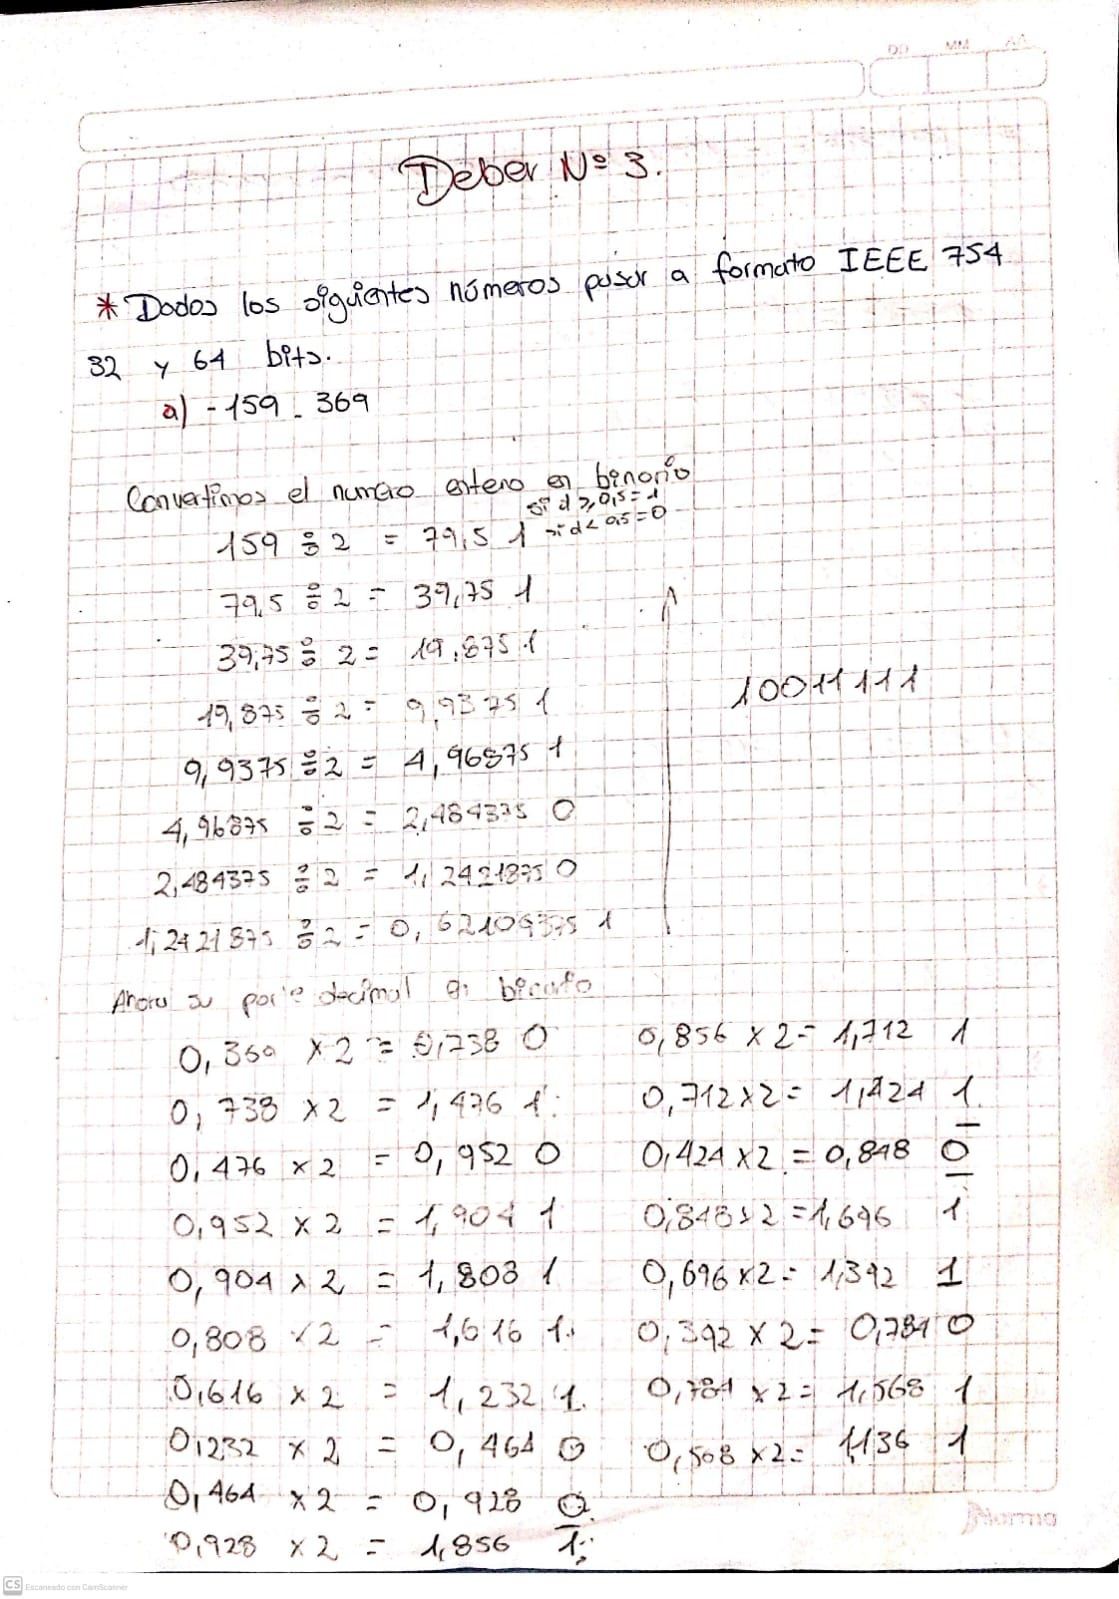
\includegraphics[width=0.95\textwidth]{inFiles/Figures/ej1.jpeg}
\end{minipage}

\vspace{0.5cm}

\begin{minipage}{0.95\textwidth}
    \raggedleft
    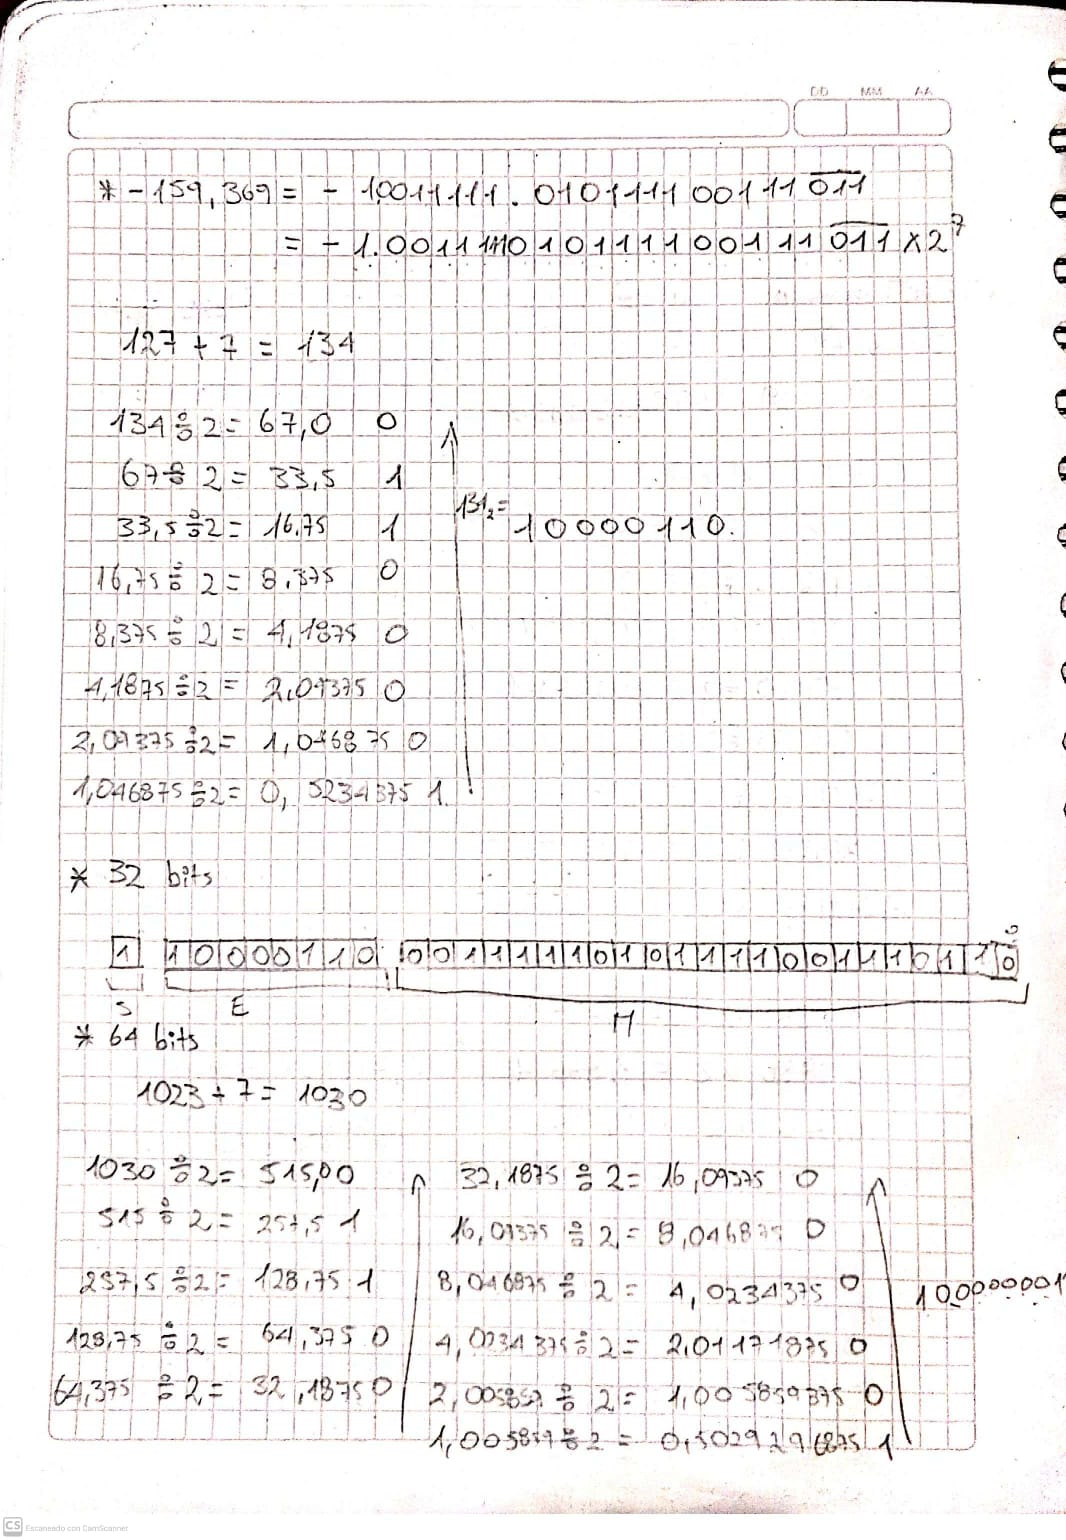
\includegraphics[width=0.95\textwidth]{inFiles/Figures/ej2.jpeg}
\end{minipage}

\vspace{0.5cm}

\begin{minipage}{0.95\textwidth}
    \raggedleft
    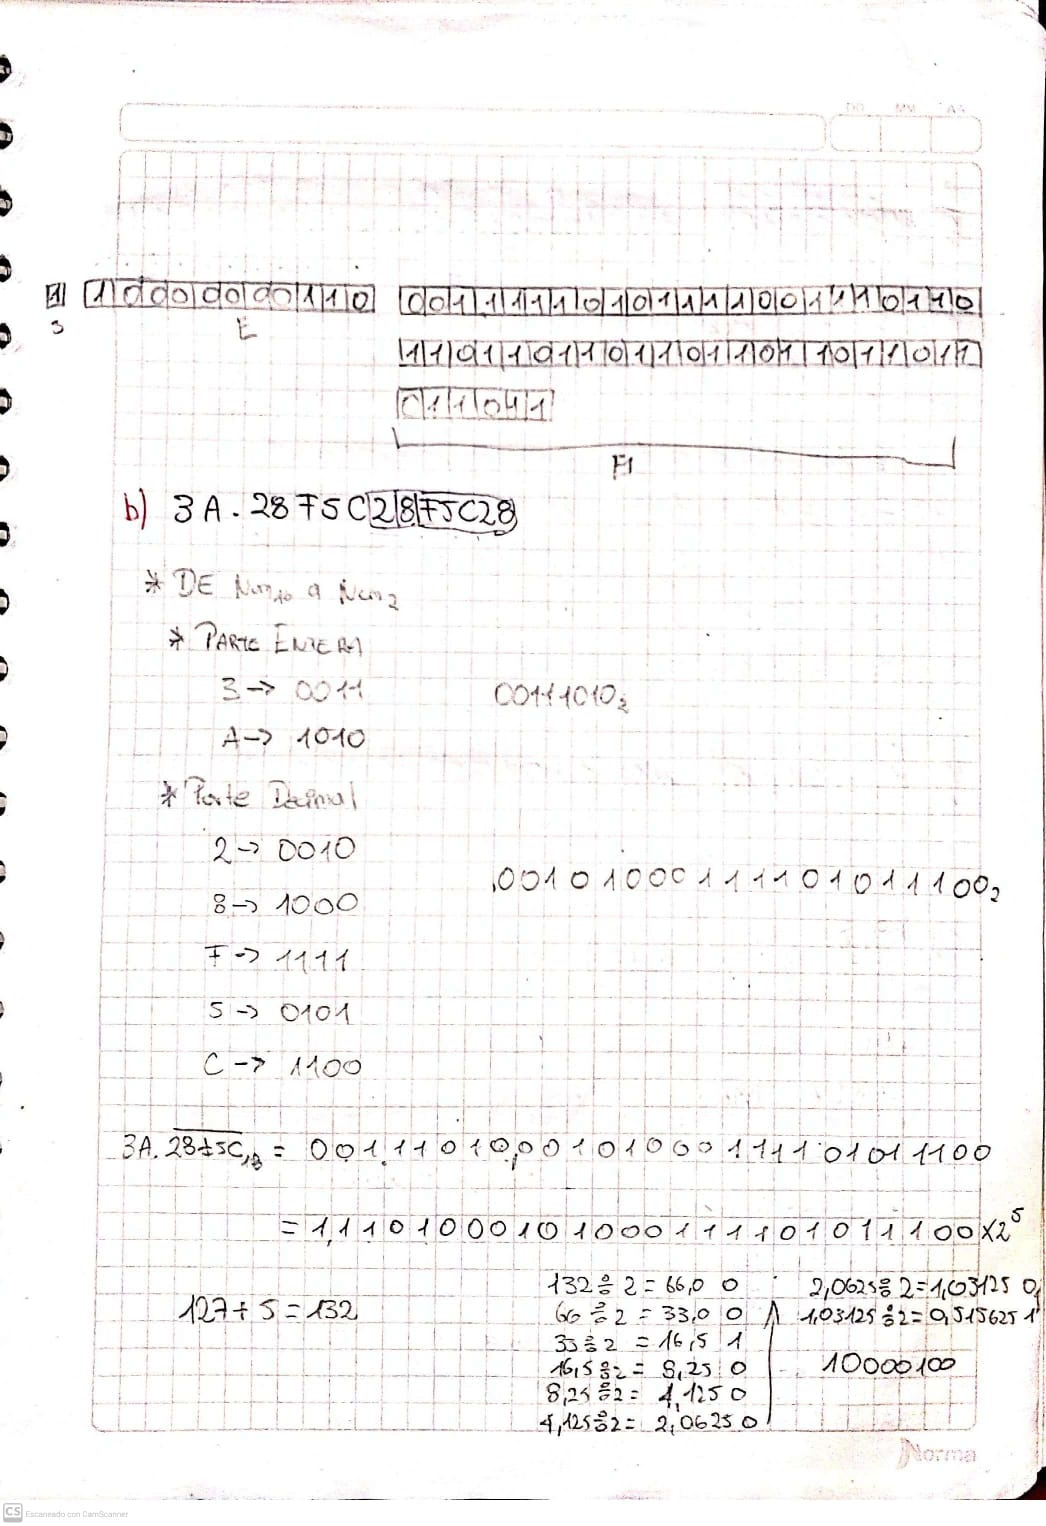
\includegraphics[width=0.95\textwidth]{inFiles/Figures/ej3.jpeg}
\end{minipage}

\vspace{0.5cm}

\begin{minipage}{0.95\textwidth}
    \raggedleft
    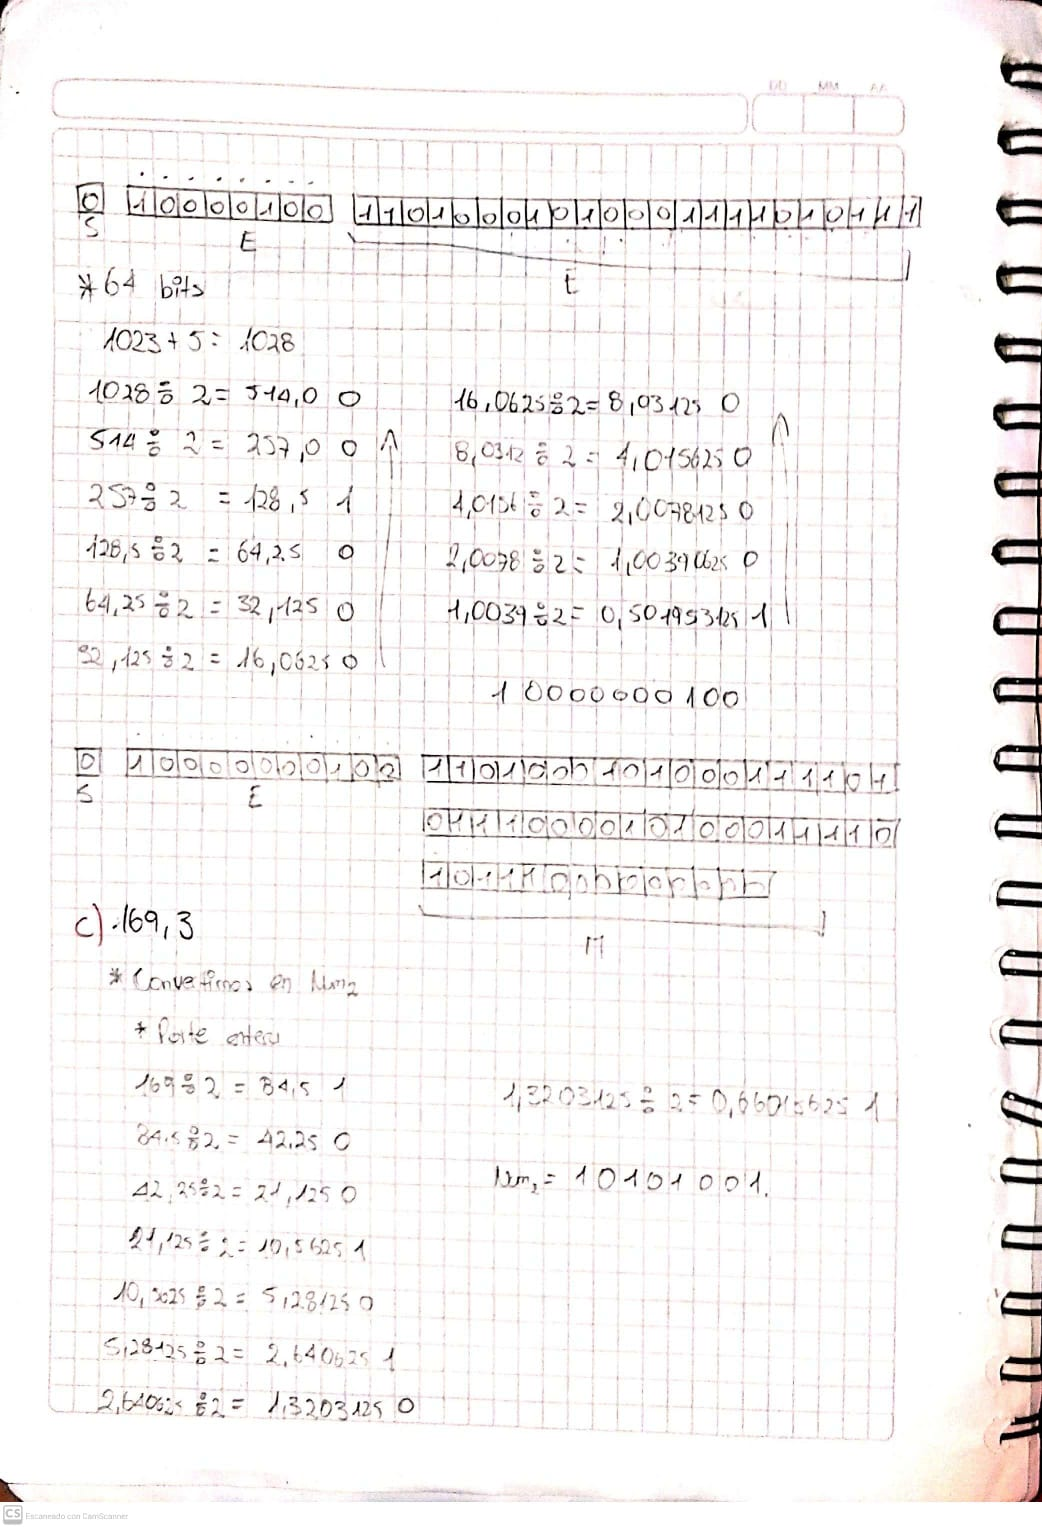
\includegraphics[width=0.95\textwidth]{inFiles/Figures/ej4.jpeg}
\end{minipage}

\vspace{0.5cm}

\begin{minipage}{0.95\textwidth}
    \raggedleft
    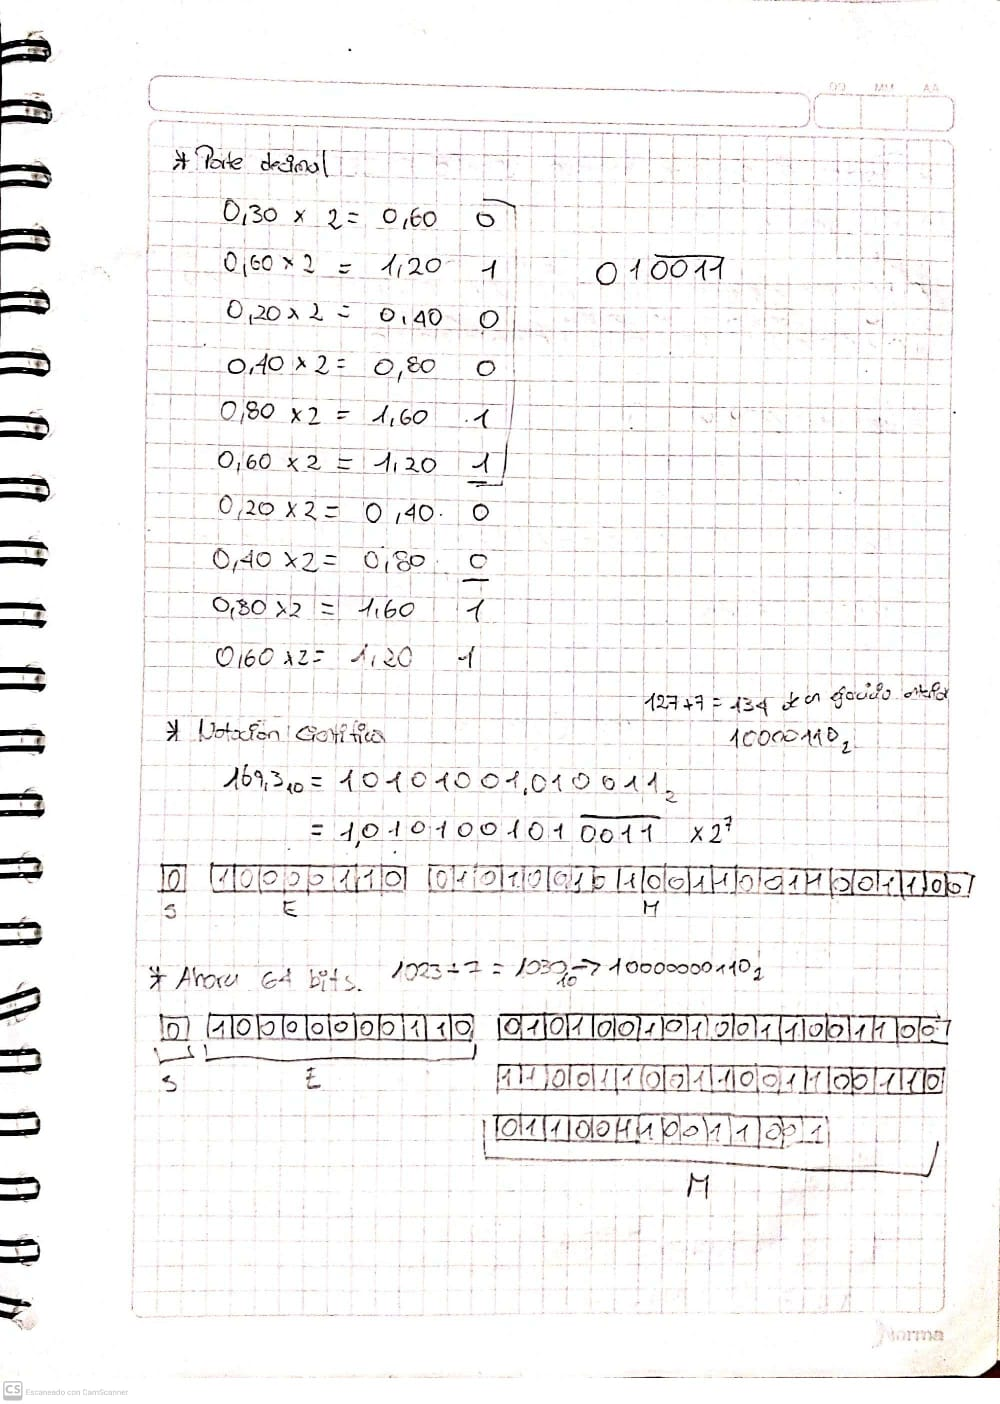
\includegraphics[width=0.95\textwidth]{inFiles/Figures/ej5.jpeg}
\end{minipage}

\vspace{0.5cm}

\begin{minipage}{0.95\textwidth}
    \raggedleft
    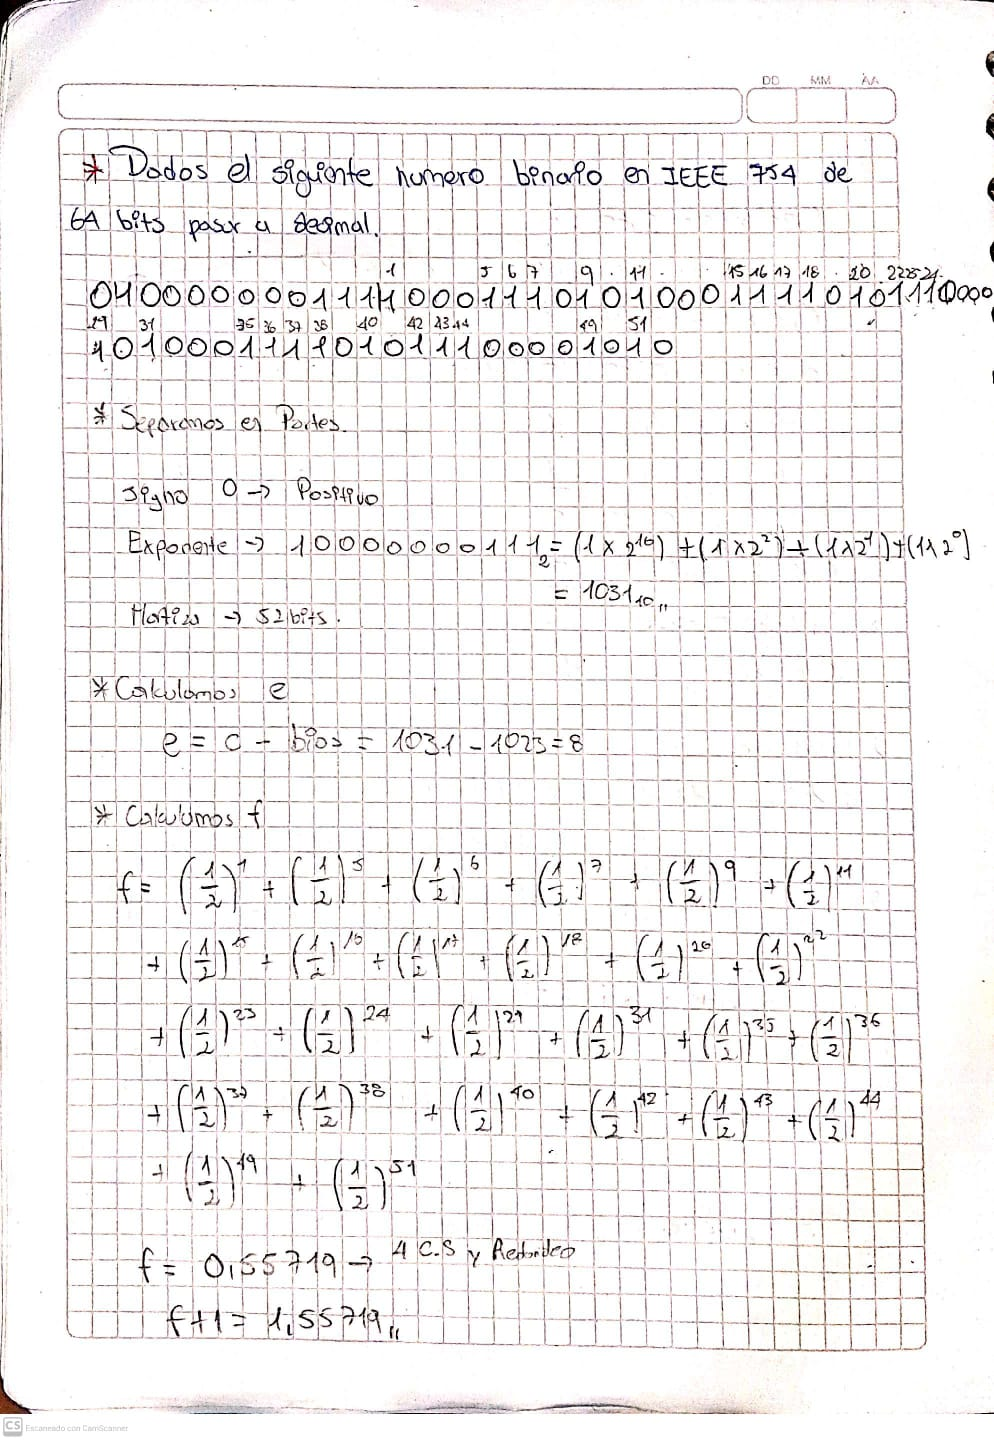
\includegraphics[width=0.95\textwidth]{inFiles/Figures/ej6.jpeg}
\end{minipage}

\vspace{0.5cm}

\begin{minipage}{0.95\textwidth}
    \raggedleft
    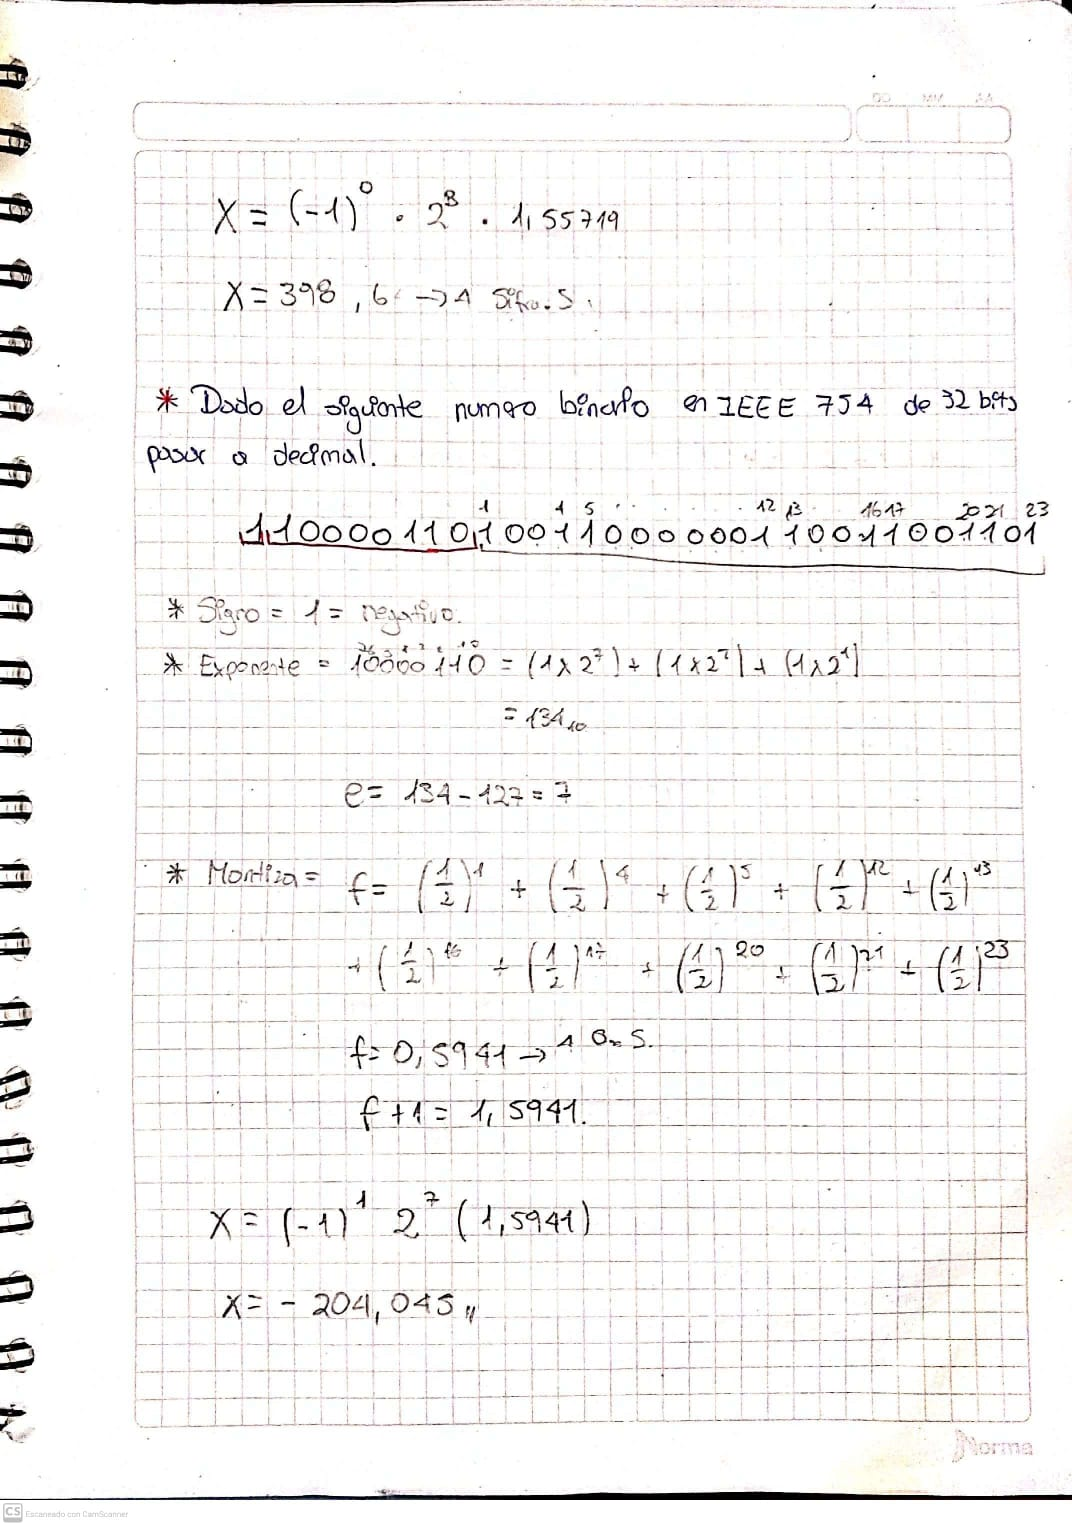
\includegraphics[width=0.95\textwidth]{inFiles/Figures/ej7.jpeg}
\end{minipage}

\vspace{3cm}


\section*{CONCLUSIONES}
\begin{itemize}
    \item {Realizar los ejercicios propuestos permitió tener un conocimiento mas profundo sobre los números en los sistemas 
    digitales usando el estándar IEEE 754 tanto en 32 bits como en 64 bits.}
\end{itemize}


\vspace{0.5cm}


\end{document}
